\documentclass[../main.tex]{subfiles}
\graphicspath{{\subfix{../images/}}}
\begin{document}
\section*{Term 2 Week 3}
\begin{enumerate}
    \item 
    Suppose \textit{r, s}, and \textit{t} are non-zero real numbers such that the polynomial \(x^2+rx+s\) has \textit{s} and \textit{t} as roots, and the polynomial \(x^2+tx+r\) has 5 as a root. Compute \(s\).\\

    \item 
    Suppose \textit{a} and \textit{b} are positive integers. Isabella and Vidur both fill up an \(a\times b\) table. Isabella fills it up with numbers \(1,2,3...ab\), putting the numbers \(1,2...b\) in the first row, \(b+1, b+2...2b\) in the second row, and so on. Vidur fills it up like a multiplication table, putting \textit{ij} in the cell in row \textit{i} and column \textit{j}.\\
    
    Examples are shown for a 3 x 4 table below:
    \begin{figure}[H]
        \centering
        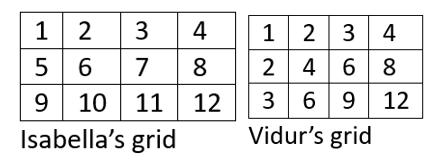
\includegraphics[width=0.3\linewidth]{images/t2w3q2.png}
    \end{figure}
    Isabella sums up the numbers in her grid, and Vidur sums up the numbers in his grid. The difference between the sums is 1200. Compute \(a+b\).\\
    
    \item 
    Given \(f(x)=x+\frac{1}{2x+\frac{1}{2x+\frac{1}{2x+...}}}\)\\

    Determine the value of \(f(99).f'(99)\).\\

    \item 
    Inside an equilateral triangle of side length 6, three congruent equilateral triangles of side length \textit{x} with sides parallel to the original equilateral triangle are arranged so that each has a vertex on a side of the larger triangle, and a vertex on another one of the smaller triangles, as shown below:\\
    \begin{figure}[H]
        \centering
        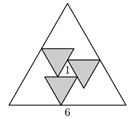
\includegraphics{images/t2w3q4.png}
    \end{figure}
    A smaller equilateral triangle formed between the three congruent equilateral triangles has side length 1. Find the length of \textit{x}.\\

    \item 
    Compute the sum of all integers \textit{n} such that \(n^2-3000\) is a perfect square.

    
\end{enumerate}

\end{document}